\subsection{Tranzityvių priklausomybių valdymas Maven sistemoje}

Vartotojo patogumui pom.xml faile būtina nurodyti tik tiesiogines jo projekto priklausomybes -
įrašant reikalingas tiesiogines priklausomybes automatiškai įrašomos ir jų priklausomybės, kitaip žinomos
kaip tranzityvios (ang. transitive) priklausomybės \cite{MAVENd}. Maven turi daug ypatybių leidžiančių patogiau valdyti
projekto tranzityvias priklausomybes.

\subsubsection{Priklausomybių mediacija}
Priklausomybių mediacija (ang. dependency mediation) yra vienas iš Maven siūlomų
funkcionalumų valdyti projekto tranzityvias priklausomybes. Tai algoritmas, nustatantis, kuri
tranzityvios priklausomybės versija turi būti atsiųsta, jeigu priklausomybių medyje aptikta keletas skirtingų
to paties artefakto versijų. Priklausomybių mediacija artefakto versiją pasirenka pagal tai, kuri artefakto
versija priklausomybių medyje yra aukščiausia. Jei tame pačiame priklausomybių medžio lygyje sutinkamos kelios
artefakto versijos, pasirenkama pirmoji paskelbta priklausomybės versija \cite{MAVENd}.

\begin{figure}[H]
    \centering
    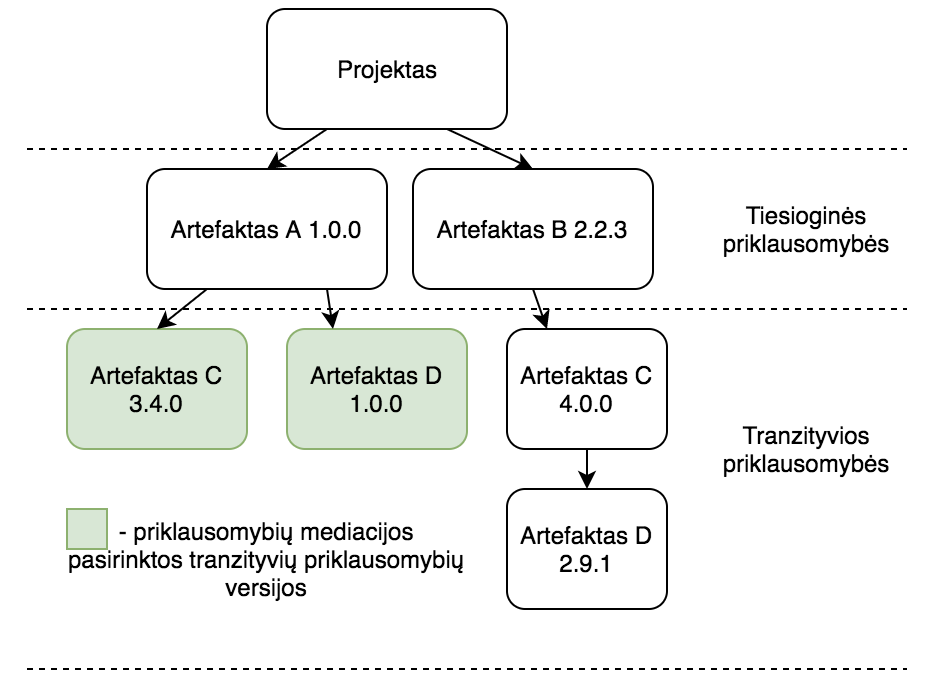
\includegraphics[width=\textwidth]{mavenv2}
    \caption{Priklausomybių mediacija}
\end{figure}

\subsubsection{Priklausomybių valdymas}
Maven siūlo ir kitus priklausomybių valdymo mechanizmus. Priklausomybių valdymas (ang. dependency management)
leidžia konkrečiai specifikuoti, kokios priklausomybių versijos bus naudojamos, jei
tos priklausomybės atsidurs tarp projekto tranzityvių priklausomybių. Tai itin paranku, jei priklausomybių
mediavimo (ang. dependency mediation) metu buvo atsiųstos ne tos versijos priklausomybės \cite{MAVENd}.

\subsubsection{Pašalintos bei pasirenkamosios priklausomybės}
Pašalintos priklausomybės (ang. excluded dependencies) suteikia galimybę uždrausti
projektui atsisiųsti tam tikrų nurodytų priklausomybių, net jei tos priklausomybės
priklauso projekto tranzityvioms priklausomybėms. Pasirenkamos priklausomybės (ang. optional dependencies) - leidžia
ignoruoti tam tikras nurodytas tranzityvias priklausomybes iki kol projekto autorius aiškiai nenurodo naudoti
šias pasirenkamas priklausomybes. Pašalintų bei pasirenkamųjų priklausomybių mechanizmai leidžia
vartotojui sumažinti projekto priklausomybių medį, taip pagreitinant projekto programinio kodo surinkimą (ang. build) \cite{MAVENd}.